\section{Task 01a}
In this exercise I will solve the one dimensional Poisson equation with Dirichlet boundary conditions by rewriting it as a set of linear equations. 

\begin{equation}
	-u''(x) = f(x),  x\in (0,1), u(0)=u(1)=0
\end{equation}

We can approximate the second order derivative of u with:

\begin{equation*}
   -\frac{v_{i+1}+v_{i-1}-2v_i}{h^2} = f_i  \hspace{0.5cm} \mathrm{for} \hspace{0.1cm} i=1,\dots, n,
\end{equation*}

This can be written as a set of linear equations almost directly:

\begin{equation*}
   -v_{i-1}+2v_i-v_{i+1} = f_i h^2  \hspace{0.5cm} \mathrm{for} \hspace{0.1cm} i=1,\dots, n,
\end{equation*}

\begin{equation*}
   -v_{0}+2v_1-v_{2} = f_1 h^2\\
\end{equation*}
\begin{equation*}
   -v_{1}+2v_2-v_{3} = f_2 h^2\\
\end{equation*}
\begin{equation*}
   -v_{2}+2v_3-v_{4} = f_3 h^2\\
\end{equation*}
\begin{equation*}
   -v_{n-2}+2v_{n-1}-v_{n} = f_{n-1} h^2\\
\end{equation*}
\begin{equation*}
   -v_{n-1}+2v_n-v_{n+1} = f_n h^2\\
\end{equation*}

$v_0$ and $v_{n+1}$ are 0, so the linear equations reduce to the following matrix form:
\[
\begin{bmatrix}
       2& -1& 0 &\dots   & \dots &0 \\
       -1 & 2 & -1 &0 &\dots &\dots \\
       0&-1 &2 & -1 & 0 & \dots \\
       & \dots   & \dots &\dots   &\dots & \dots \\
       0&\dots   &  &-1 &2& -1 \\
       0&\dots    &  & 0  &-1 & 2 \\
\end{bmatrix}
\begin{bmatrix}
	v_1 \\
	v_2 \\
	v_3 \\
	\vdots \\
	v_{n-1} \\
	v_n \\                      
\end{bmatrix} = 
h^2
\begin{bmatrix}
	f_1 \\
	f_2 \\
	f_3 \\
	\vdots \\
	f_{n-1} \\
	f_n \\                      
\end{bmatrix}
\]

This is the same form of 
\begin{equation*}
   \mathbf{A}\mathbf{v} = \tilde{\mathbf{b}},
\end{equation*}

\section{Task 01b}
In this exercise I want to find a general algorithm for solving this set of equations with different values for the matrix elements by using decomposition and forward substitution and backward substitution. Let the tridiagonal matrix have elements $a_i$, $b_i$ and $c_i$\\

For clarity replace $'\tilde{b}'$ with $'d'$
\begin{equation*}
   a_{i-1} v_{i-1} + b_i v_i + c_i v_{i+1} = d_i  \hspace{0.5cm} \mathrm{for} \hspace{0.1cm} i=1,\dots, n,
\end{equation*}

where
$v_0 = v_{n+1} = a_0 = a_{n} = c_n = 0$\\

\begin{gather*}
   b_1 v_1 + c_1 v_{2} = d_1\\
   a_{1} v_{1} + b_2 v_2 + c_2 v_{3} = d_2\\
   a_{2} v_{2} + b_3 v_3 + c_3 v_{4} = d_3\\
   \vdots\\
   a_{n-2} v_{n-2} + b_{n-1} v_{n-1} + c_{n-1} v_{n} = d_{n-1}\\
   a_{n-1} v_{n-1}+b_{n} v_{n} = d_{n}\\
\end{gather*}

Methodology: Reduce the tridiagonal matrix to an upper diagonal matrix by decomposition, forwards substitution and backward substitution.
Modifying equation 2 with equation 1 to eliminate $v_1$\\
Equation 2 * b1 - equation 1 *a1: \\

\[
\begin{bmatrix}
     b_1 & c_1     & 0     & \dots    & \dots   & \dots    & \| & d_1 \\
     a_1 & b_2     & c_2   & \dots    & \dots   & \dots    & \| & d_2 \\
         & a_2     & b_3   & c_3      & \dots   & \dots    & \| & d_3 \\
         & \dots   & \dots & \dots    & \dots   & \dots    & \| & \dots \\
         &         &       & a_{n-2}  & b_{n-1} & c_{n-1}  & \| & d_{n-1} \\
         &         &       &          & a_{n-1} & b_n      & \| & d_n \\
\end{bmatrix}  
\]

Equation 1 times $a_1$ and equation 2 times $b_1$\\
\[
\begin{bmatrix}
     a_1 b_1 & a_1 c_1     & 0     & \dots    & \dots   & \dots    & \| & a_1 d_1 \\
     b_1 a_1 & b_1 b_2     & b_1 c_2   & \dots    & \dots   & \dots    & \| & b_1 d_2 \\
         & a_2     & b_3   & c_3      & \dots   & \dots    & \| & d_3 \\
         & \dots   & \dots & \dots    & \dots   & \dots    & \| & \dots \\
         &         &       & a_{n-2}  & b_{n-1} & c_{n-1}  & \| & d_{n-1} \\
         &         &       &          & a_{n-1} & b_n      & \| & d_n \\
\end{bmatrix}  
\]

Equation 2 - equation 1\\
\[
\begin{bmatrix}
     b_1 & c_1                   & 0     & \dots    & \dots   & \dots    & \| & d_1 \\
     0   & b_1 b_2 - a_1 c_1     & b_1 c_2   & \dots    & \dots   & \dots    & \| & b_1 d_2 - a_1 d_1 \\
         & a_2                   & b_3   & c_3      & \dots   & \dots    & \| & d_3 \\
         & \dots                 & \dots & \dots    & \dots   & \dots    & \| & \dots \\
         &                       &       & a_{n-2}  & b_{n-1} & c_{n-1}  & \| & d_{n-1} \\
         &                       &       &          & a_{n-1} & b_n      & \| & d_n \\
\end{bmatrix}  
\]

$\tilde{b_2} = b_1 b_2 - a_1 c_1$ \\
$\tilde{c_2} = b_1 c_2$ \\
$\tilde{d_2} = b_1 d_2 - a_1 d_1$ \\

\[
\begin{bmatrix}
     b_1 & c_1                   & 0     & \dots    & \dots   & \dots    & \| & d_1 \\
     0   & \tilde{b_2} & \tilde{c_2}   & \dots    & \dots   & \dots    & \| & \tilde{d_2} \\
         & a_2                   & b_3   & c_3      & \dots   & \dots    & \| & d_3 \\
         & \dots                 & \dots & \dots    & \dots   & \dots    & \| & \dots \\
         &                       &       & a_{n-2}  & b_{n-1} & c_{n-1}  & \| & d_{n-1} \\
         &                       &       &          & a_{n-1} & b_n      & \| & d_n \\
\end{bmatrix}  
\]

Equation 2 times $a_2$ and equation 3 times $\tilde{b_2}$\\

\[
\begin{bmatrix}
     b_1 & c_1                   & 0     & \dots    & \dots   & \dots    & \| & d_1 \\
     0   & a_2 \tilde{b_2}       & a_2 \tilde{c_2}   & \dots    & \dots   & \dots    & \| & a_2 \tilde{d_2} \\
         & \tilde{b_2} a_2       & \tilde{b_2} b_3   & \tilde{b_2} c_3      & \dots   & \dots    & \| & \tilde{b_2} d_3 \\
         & \dots                 & \dots & \dots    & \dots   & \dots    & \| & \dots \\
         &                       &       & a_{n-2}  & b_{n-1} & c_{n-1}  & \| & d_{n-1} \\
         &                       &       &          & a_{n-1} & b_n      & \| & d_n \\
\end{bmatrix}  
\]

Equation 3 -equation 2: \\

\[
\begin{bmatrix}
     b_1 & c_1                   & 0     & \dots    & \dots   & \dots    & \| & d_1 \\
     0   & a_2 \tilde{b_2} & a_2 \tilde{c_2}   & \dots    & \dots   & \dots    & \| & a_2 \tilde{d_2} \\
         & 0                   & \tilde{b_2} b_3 - a_2 \tilde{c_2}  & \tilde{b_2} c_3      & \dots   & \dots    & \| & \tilde{b_2} d_3 - a_2 \tilde{d_2}\\
         & \dots                 & \dots & \dots    & \dots   & \dots    & \| & \dots \\
         &                       &       & a_{n-2}  & b_{n-1} & c_{n-1}  & \| & d_{n-1} \\
         &                       &       &          & a_{n-1} & b_n      & \| & d_n \\
\end{bmatrix}  
\]

$\tilde{b_3} = \tilde{b_2} b_3 - a_2 \tilde{c_2}$ \\
$\tilde{c_3} = \tilde{b_2} c_3$ \\
$\tilde{d_3} = \tilde{b_2} d_3 - a_2 \tilde{d_2}$ \\

By examining the procedure, the modified coefficients notated with tildes may be defined recursively:\\

\begin{gather*}
	\tilde{a_i} = 0 \\
	\tilde{b_1} = b_1 \\
	\tilde{b_i} = b_i \tilde{b_{i-1}} - a_{i-1} \tilde{c_{i-1}} \\
	\tilde{c_1} = c_1 \\
	\tilde{c_i} = \tilde{b_{i-1}} c_i \\
	\tilde{d_1} = d_1  \\
	\tilde{d_i} = \tilde{b_{i-1}} d_i - a_{i-1} \tilde{d_{i-1}} \\
\end{gather*}

To further hasten the solution process, $\tilde{d_i}$ may be divided out if there is no division by zero risk. The newer modified coefficients each notated with a hat will be:\\

\begin{gather*}
	\hat{a_i} = 0 \\
	\hat{b_i} = 1 \\
	\hat{c_1} = \frac{c_1}{b_1} \\
	\hat{c_i} = \frac{c_i}{b_i - a_{i-1} \hat{c_{i-1}}} \\
	\hat{d_1} = \frac{d_1}{b_1}  \\
	\hat{d_i} = \frac{ d_i - a_{i-1} \hat{d_{i-1}}}{b_i - a_{i-1} \hat{c_{i-1}}} \\
\end{gather*}

This gives the following system with the same unknowns and coefficients defined in terms of the original ones above: \\

$v_i + \hat{c_i} v_{i+1} = \hat{d_i}$

$v_n = \hat{d_n}$

The last equation involves only one unknown. Solving it in turn reduces the next last equation to one unknown. This backward substitution can be used to find all of the unknowns: \\
$v_n = \hat{d_n}$  \\
$v_i + \hat{c_i} v_{i+1} = \hat{d_i}$ for $i = n-1, n-2, \ldots, 1$ \\

Floating point operations: \\

For calculating $\hat{c_i}$ we need $3(n-2)+1$ flops. \\
For calculating $\hat{d_i}$ we need $5(n-1)+1$ flops. \\
For back substitution we need $2(n-1)+1$ flops. \\

However the denominator is the same for both $\hat{c_i}$ and $\hat{d_i}$. Thus the calculation of the denominator only has to be carried out once. Therefore we can subtract 2(n-2) flops from the total number of flops.


In total to solve the problem we need $7(n-1)+3(n-2)-2(n-2)+3 = 8(n-1)+2$ flops. \\


\FloatBarrier
\begin{figure}[!ht]
\centering
\FloatBarrier
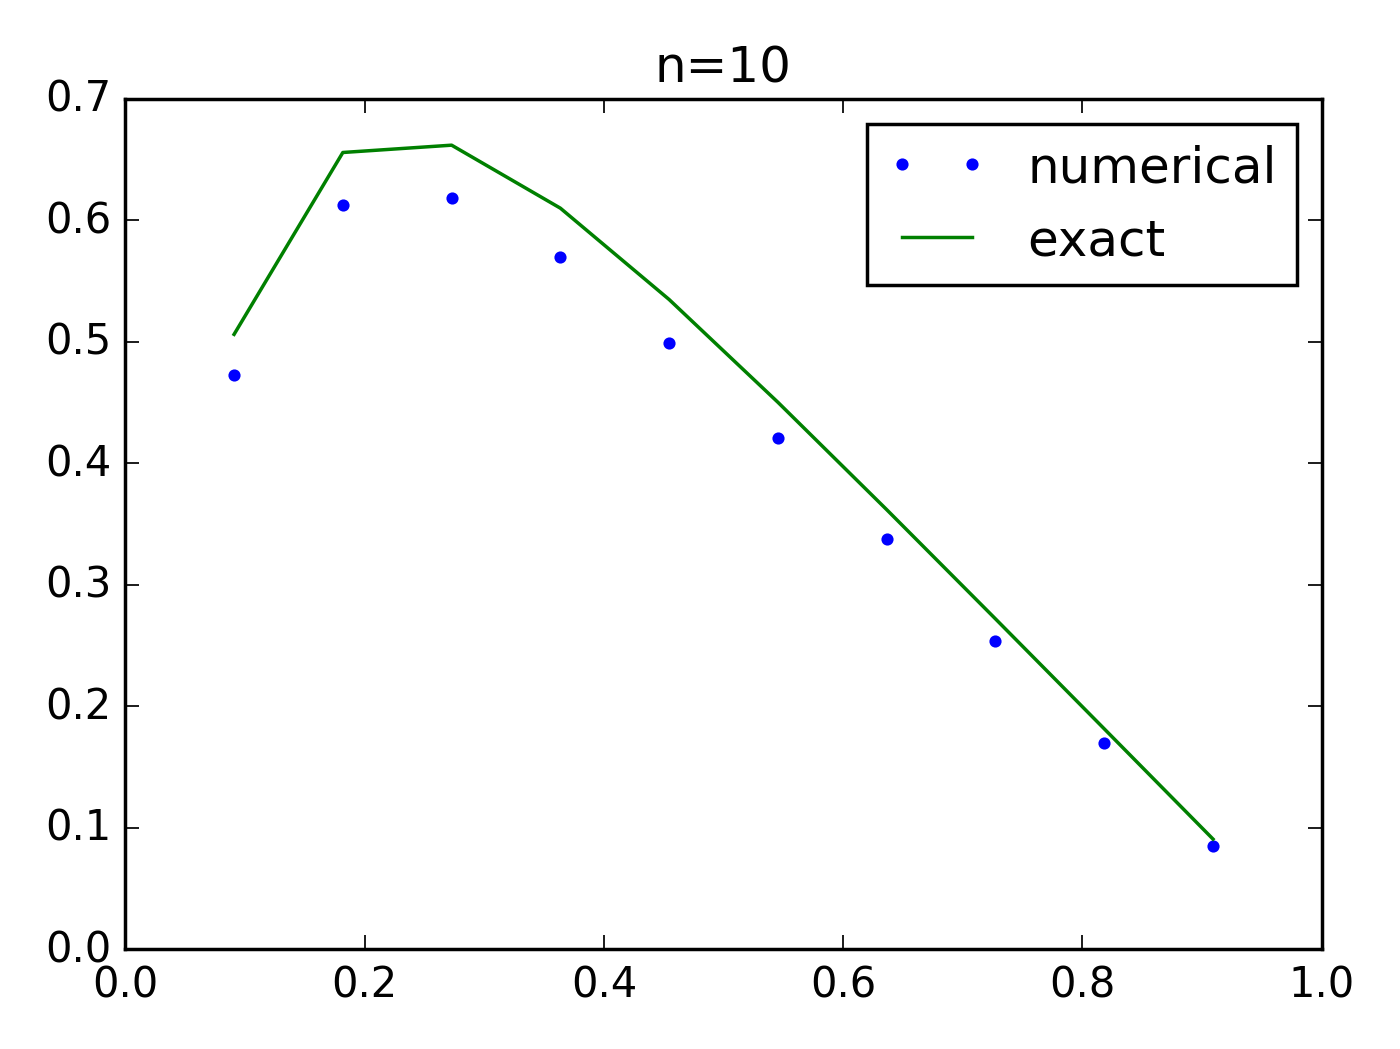
\includegraphics[width=0.32\textwidth]{task1b_n10.png}
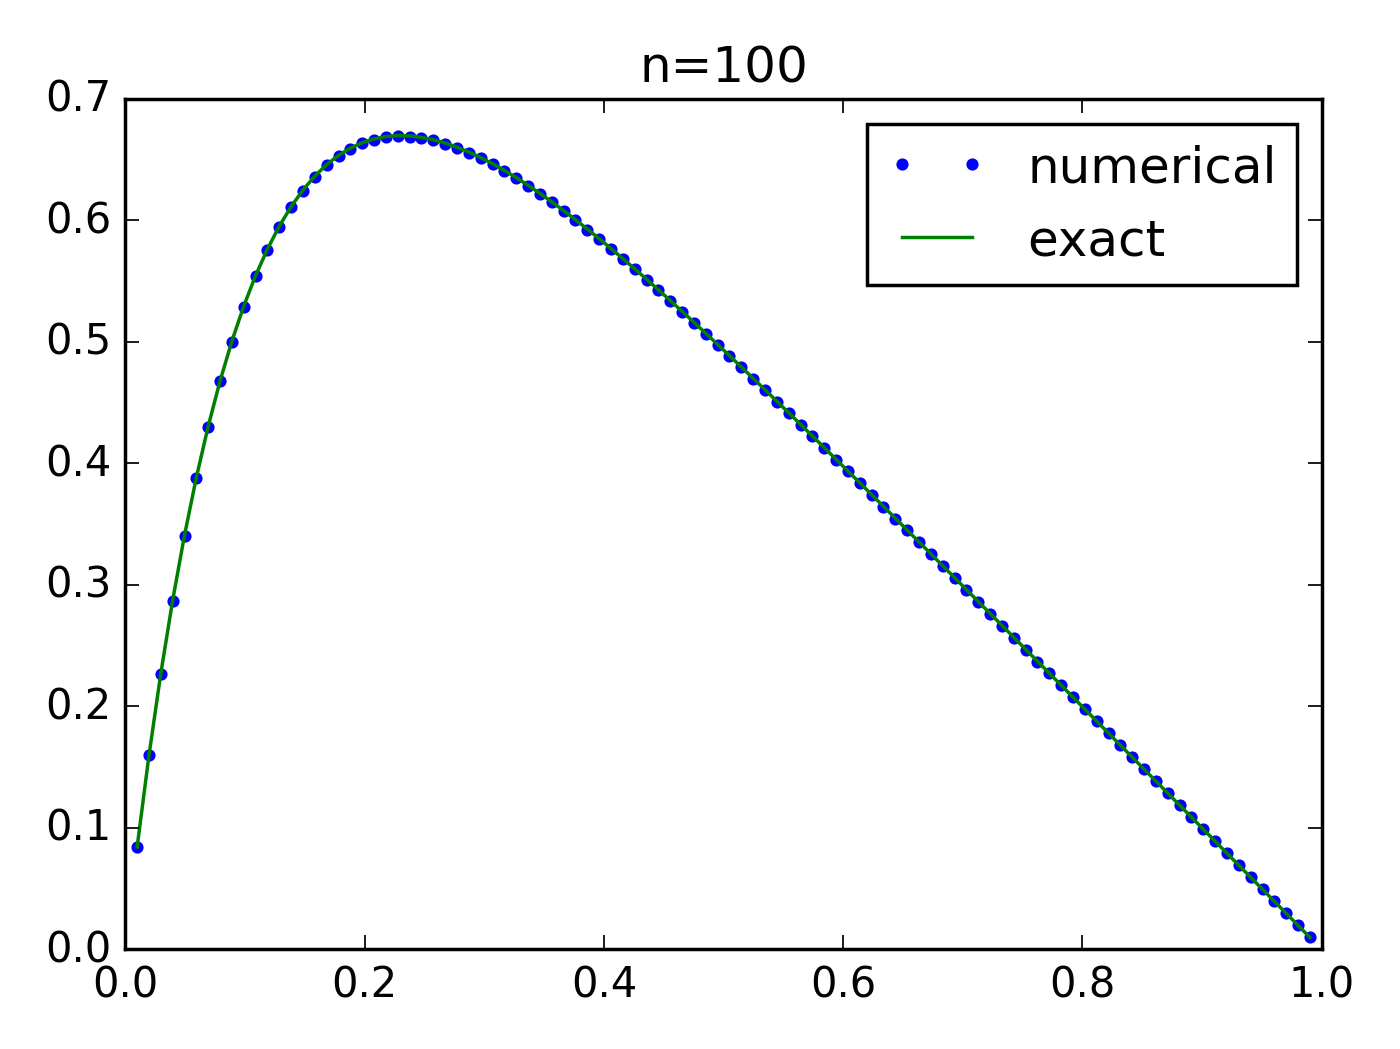
\includegraphics[width=0.32\textwidth]{task1b_n100.png}
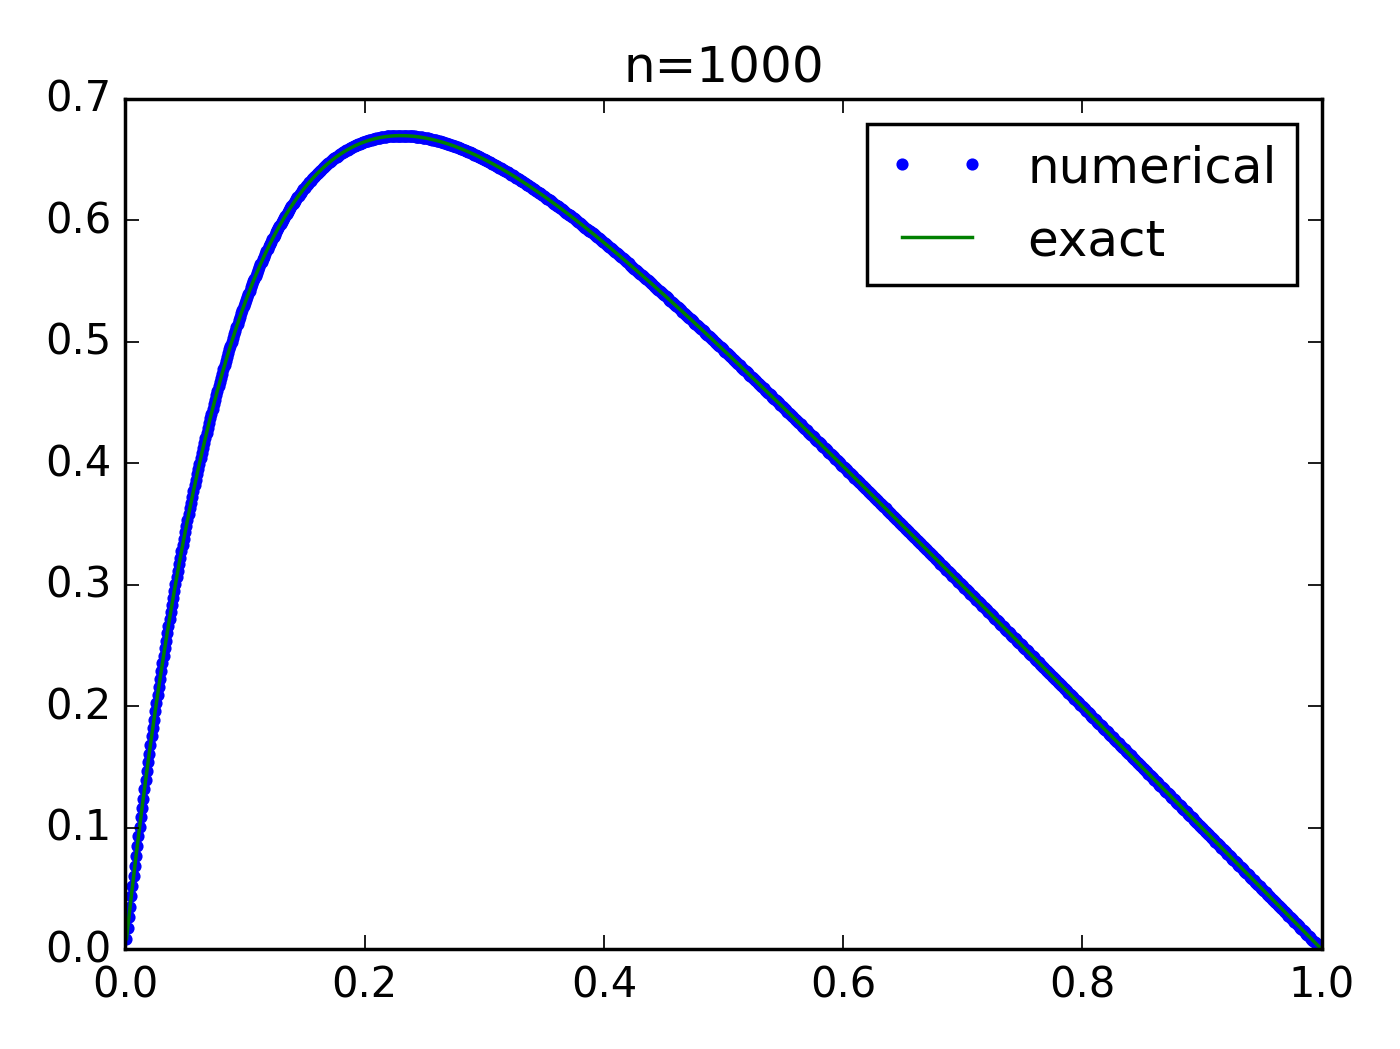
\includegraphics[width=0.32\textwidth]{task1b_n1000.png}
\caption{Solving the Poisson equation numerically and exact with grid size n =10,100,1000}
\label{fig:Poisson}
\end{figure}
\FloatBarrier

From figure~\ref{fig:Poisson} I can see that the numerical solution approaches the exact solution for more grid points. \\


\section{Task 01c}

Assuming identical matrix elements along the diagonal and identical  but different values for the non-diagonal elements. This means that the $a_i =c_i =-1$ and $b_i =2$. Substituting this result into the solution we found in project 1b we get:
\begin{gather*}
	\hat{a_i} = 0 \\
	\hat{b_i} = 1 \\
	\hat{c_1} = -0.5 \\
	\hat{c_i} = \frac{-1}{2 + \hat{c_{i-1}}} \\
	\hat{d_1} = \frac{d_1}{2}  \\
	\hat{d_i} = \frac{d_i + \hat{d_{i-1}}}{2 + \hat{c_{i-1}}} \\
\end{gather*}


Floating point operations specific: \\

For calculating $\hat{c_i}$ we need $2(n-2)$ flops. \\
For calculating $\hat{d_i}$ we need $3(n-1)+1$ flops. \\
Back substitution does not change so it's the same is in 1b, we need $2(n-1)+1$ flops. \\

The denominator is the same for both $\hat{c_i}$ and $\hat{d_i}$. Thus the calculation of the denominator only has to be carried out once. Therefore we can subtract (n-2) flops from the total number of flops.


In total to solve the specific problem we need $5(n-1)+2(n-2)-(n-2)+2 = 6(n-1)+1$ flops. \\

Running the program to check for CPU time for both the general and the specific case I got very similar results the first time. General case gave  a time of: 7.62825565887. The specific case gave a time of
7.512299363. This is probably because pure Python code has more overhead than compiled languages like C++ or Fortran, minimizing the importance of flops. Therefore I tried to import numba, which compiles the code just in time. This resulted in a time for the general case of; 0.515605151976 seconds, and for the specific case:
0.309811743968 seconds. Comparing the flops to the running times, I get for Flops: $(9(n-1)+2)/(6(n-1)+1) \approx 1.5$ and for running times: $0.515605151976/0.309811743968 \approx 1.65$\\


\section{Task 01d}
In this exercise I want to check for truncation errors in the calculations.\\

Here I made a function that extracts the maximum relative error for each step length. The results of the calculations are shown in figure~\ref{fig:Error_poisson}.\\

\FloatBarrier
\begin{figure}[!ht]
\centering
\FloatBarrier
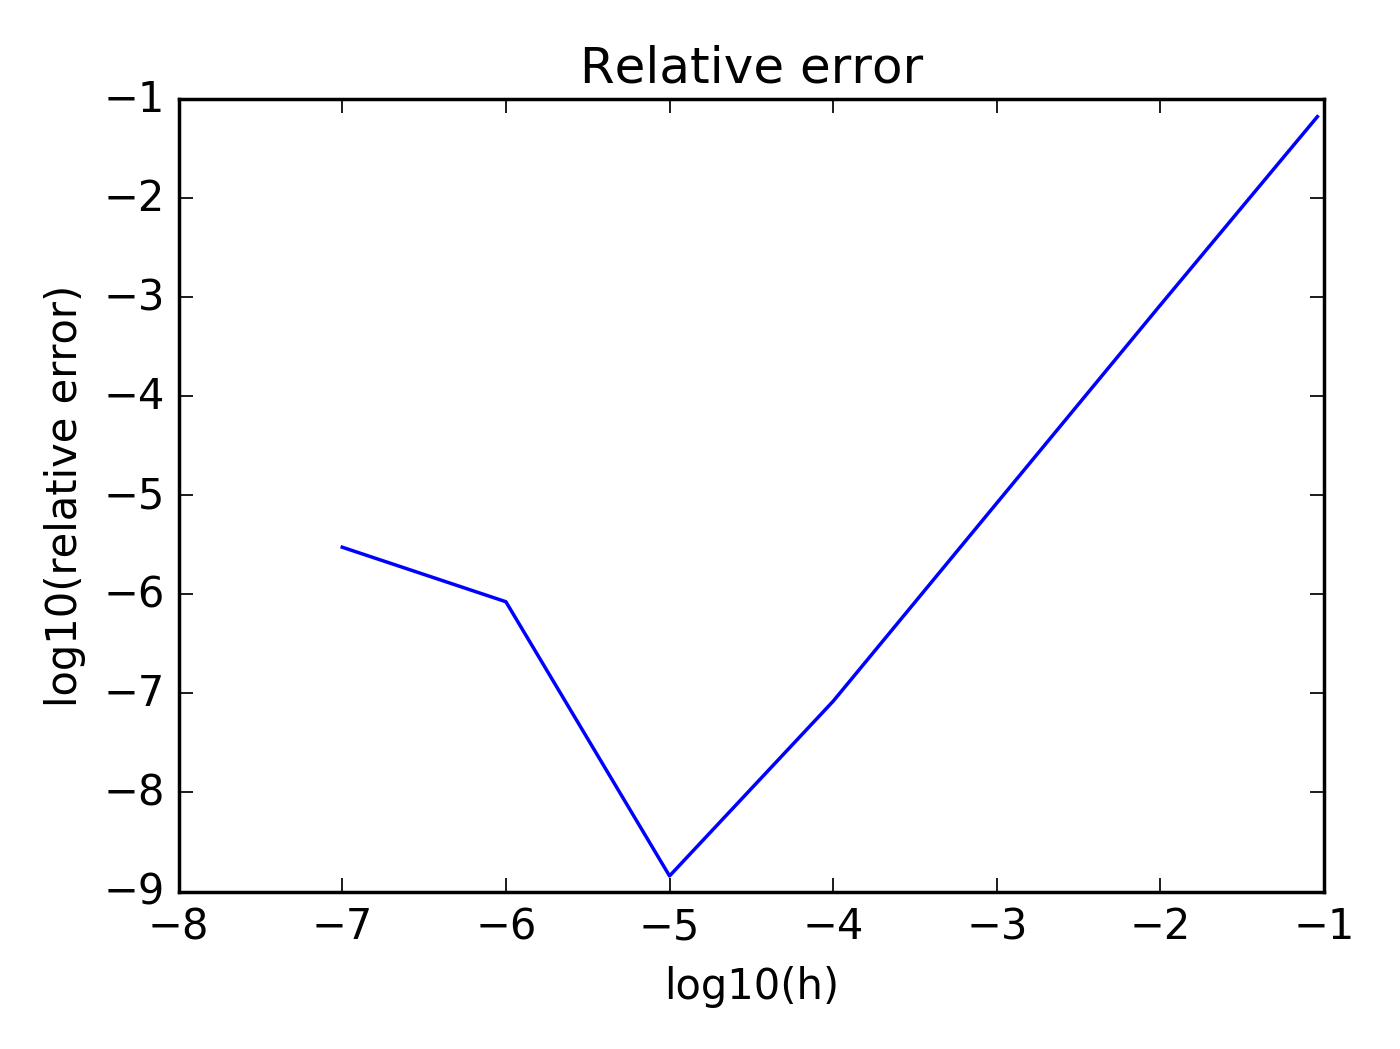
\includegraphics[width=0.45\textwidth]{error.png}

\caption{Computing the relative error of the numerical solution to the Poisson equation for grid sizes n =10, 100, 1000, 10000, 100000, 1000000, 10000000}
\label{fig:Error_poisson}
\end{figure}
\FloatBarrier

In the figure~\ref{fig:Error_poisson} I can see that the error declines until h reaches about $10^{-5}$. Decreasing the step size beyond this value results in increased truncation errors.\\


\section{Task 01e}
Flops of LU decomposition goes like $O(n^2)$ when trying to solve the set of linear equations.

Trying to run the LU decomposition for a matrix of size $10^{10}$ does not work because I have too little memory space.

\FloatBarrier
\begin{table}[!ht]
\centering
\begin{tabular}{|c|c|c|c|}
\hline 
n & tridiagonal specific & tridiagonal & LU \\ 
\hline 
10 & 0.000204 & 0.000177 & 0.002522 \\ 
\hline 
100 & 0.000212 & 0.000199 & 0.002558 \\ 
\hline 
1000 & 0.000478 & 0.000557 & 0.299024 \\ 
\hline 
2000 & 0.000293 & 0.000516 & 1.664050 \\
\hline 

\label{Runtimes for various methods of decomposition}
\end{tabular} 
\caption{Runtimes in seconds for various methods of decomposition}
\end{table}
\FloatBarrier

For tridiagonal specific flops goes like $O(6n)$. For tridiagonal flops goes like $O(9n)$. LU decomposition flops goes like $O(n^2)$. From the runtimes I can see in \ref{Runtimes for various methods of decomposition} that the two first grows linearly within errors, while the LU decomposition grows quadratically.\\


\section{Comments}
In general the exercise was useful, but I realize that I could have written the report better. I have just gotten started with github, so I attached the program code, like I have done in projects I have done in the past. I hand in the exercise a bit late, because I was abroad until recently after agreement with Morten. It would be great to get some feedback on some of the report outlines, and maybe a tip on where or how I could implement further tests in my program. 